\documentclass[12pt, letterpaper, titlepage]{article}
\usepackage{graphicx}
\usepackage{hyperref}
\usepackage[margin=1in]{geometry}

\hypersetup{colorlinks = true, linkcolor = blue, citecolor=blue, urlcolor = blue}

\title{CSE 5825: Bayesian Machine Learning Project Proposal}
\author{Owen Fiore and Jared Sullivan}

\begin{document}
\maketitle

\section{Working with data}
\subsection{Question 1}
We have collected data from the last 5 season from Basketball Reference and converted it to a csv. However, we may include more data from previous years as appropriate.  We chose recent data due to concerns about changing of league strategies and overall change
in how basketball is played in the NBA.  More now that ever, players have tried
to vary their skill set to be more versatile and thus adaptable to other teams.
The data is fairly exhaustive, as it contains every important statistic tracked
in basketball in addition to many advanced statistics that have been developed
in recent years by basketball statisticians to try and gauge player performance.
In terms of biases of the data, there may be issues with how recent it is, and
we may want to include more data to increase sample size. 


An important confounder we need to consider is what is known as “garbage time”
in basketball and this generally refers to the minutes played at the end of the game where one team has such a lead that often both teams will take out their starters
and replace them with their bench players.  These bench players may get
inflated statistics from playing against other bench players and may seem
like they are better than they actually are.  That is one reason we tried to
look at statistics on a per-game basis, because statistics generated per
36 minutes or 100 possessions (two commonly used basketball time
frames roughly equal to the average number of minutes a quality starter
would play and the number of possessions a team averages in a game)
may be biased towards worse players. However, we still need to have a
sufficiently sized data set meaning that we are going to be forced to include
players who do not play a lot each game.  As coaches play the best players
most of the game, typically seven to nine players on each team get meaningful minutes
in standard regular season games.


\subsection{Question 2}
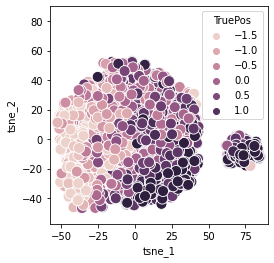
\includegraphics{tSNE}
The t-SNE or t-distributed stochastic neighbor embedding plot shows that across several
important variables such as rebounds, assists, field goal percentages there are differences across positions.  Many of the points on the left represent guards as they are colored in
lightly, while the points on the right represent the big men: power forwards and
centers. As t-SNE is a low dimensional representation of a high dimensional clustering,
our attempt to be able to separate players by position was successful. For our t-SNE
plot we noticed that there is one cluster filled with mostly centers that fall outside
the normal space of the players. This could be due to a hidden variable we have not
accounted for yet, and it will require further investigation. One plausible explanation is that center has a more distinct play style and that could be causing the isolation.


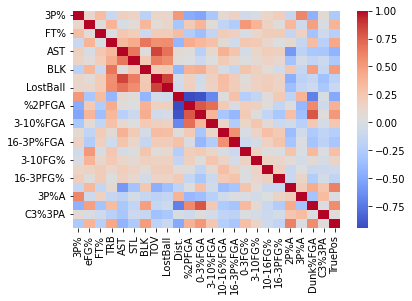
\includegraphics{heatmap}

For the correlation matrix heatmap it was helpful in demonstrating which of our variables are highly correlated with each other. A big part of our feature selection is trying to find what features model a certain relationship and how those features interact with each other in high dimensional space. For example if we clustered based on player positions which originally had 5 features describing it then it would be 5 times the weight in a euclidean distance when finding how different two points are. The heatmap shows that where a player shoots from on average and their field goal percent averages at that distance has a heavy correlation. This was to be expected, and we will take this into account moving forward if we want to implement more feature selection.

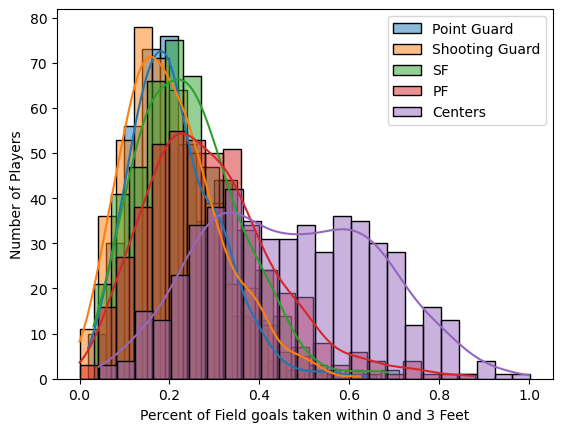
\includegraphics{0-3FT}
The last graph shows for each position, the distribution of players who took field goals within 0 and 3 feet.  For example, 0.2 on the x-axis means that 20\% of a player’s shots were from 0-3 feet, and if y = 20, then 20 players of a particular position took 20\% of their shots from 0-3 feet.  What is clear is that the center position had by far the most variation, indicating there are centers who take very few shots near the basket, and some that take nearly all of their shots at the basket.  This suggests that there are major differences between Centers and where they shoot the ball from, but the differences for point guards is clearly smaller.

\section{Thinking about models}
\subsection{Question 1}
The observed variables in the data are player statistics that include shooting
percentages, how efficient players were, defensive contributions, and where
players shot from.  There are many columns of the data that are calculated from
other columns, but we chose to include these as they are informative.  For
example, field goal percent is the player's made field goals divided by their
field goal attempts.  Looking at field goal percent by itself can be helpful, but
there are players in the NBA who may have high field goal percentages because
they do not shoot a lot and when they do, their shots are mostly dunks which are
generally made shots.  Essentially they do not attempt many shots and the shots
they do attempt are easy to make. We also know that the players who play the most
play time will impose less noise on the data set than players who don’t.

\subsection{Question 2}
One hidden variable we are going to implement is a scaled position estimate. We
have the estimates of the percent at each position a player played during the
season.  Using this we can create a scale from 1 to 5 of the five positions.  For
example a player who is at 1.00 is a pure point guard, 5.00 is a pure center,
but 1.50 is a player halfway between point guard and shooting guard.  We are able
to do this because basketball player positions are ordinal. When we implemented 
this hidden variable on the tSNE plot we created we could see a visible gradient across 
the graph. This may indicate that the hidden variable of scaled position estimate has some influence on the data.

\subsection{Question 3}
We will explore three main hypotheses in this project, the first of which is there are
ways of analyzing each clustering of different players in the NBA.  Once we do this, we
can go within each cluster and see if we observe differences within that position. 
This is our second hypothesis and goes back to the conversation about why Steph Curry
and De'Aaron Fox are different players and determining if there exists archetypes
within a position, potentially using auto-correlation.  Lastly, we could attempt to use
those results to try to come up with a model that predicts success, potentially using
Bayesian regression, to determine if there are combinations of players that would be
more successful.  We would analyze championship teams to try and determine what
combinations of archetypes are beneficial to team success.

\end{document}